\chapter{Results from Local Analysis}
\label{appendix:C}

\begin{figure}[H]
\subfloat[Tension in conductor \label{fig:f1}]
  {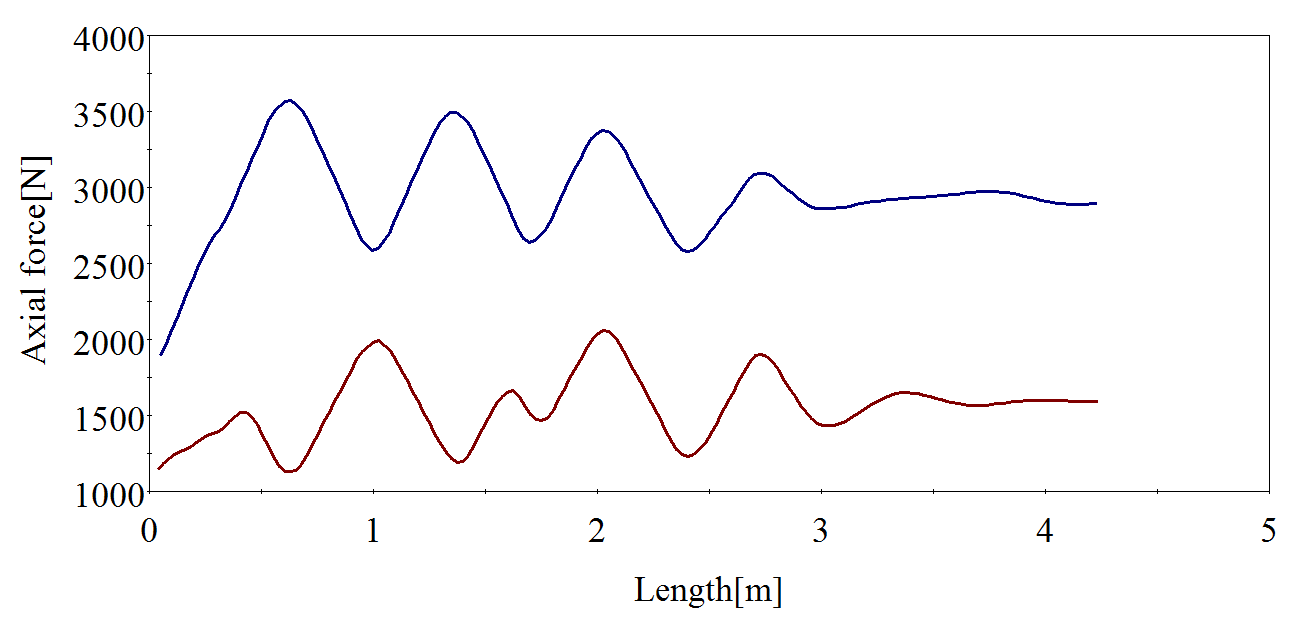
\includegraphics[width=.45\linewidth]{figures/f1}}\hfill
\subfloat[Curvature in conductor \label{fig:c1}]
  {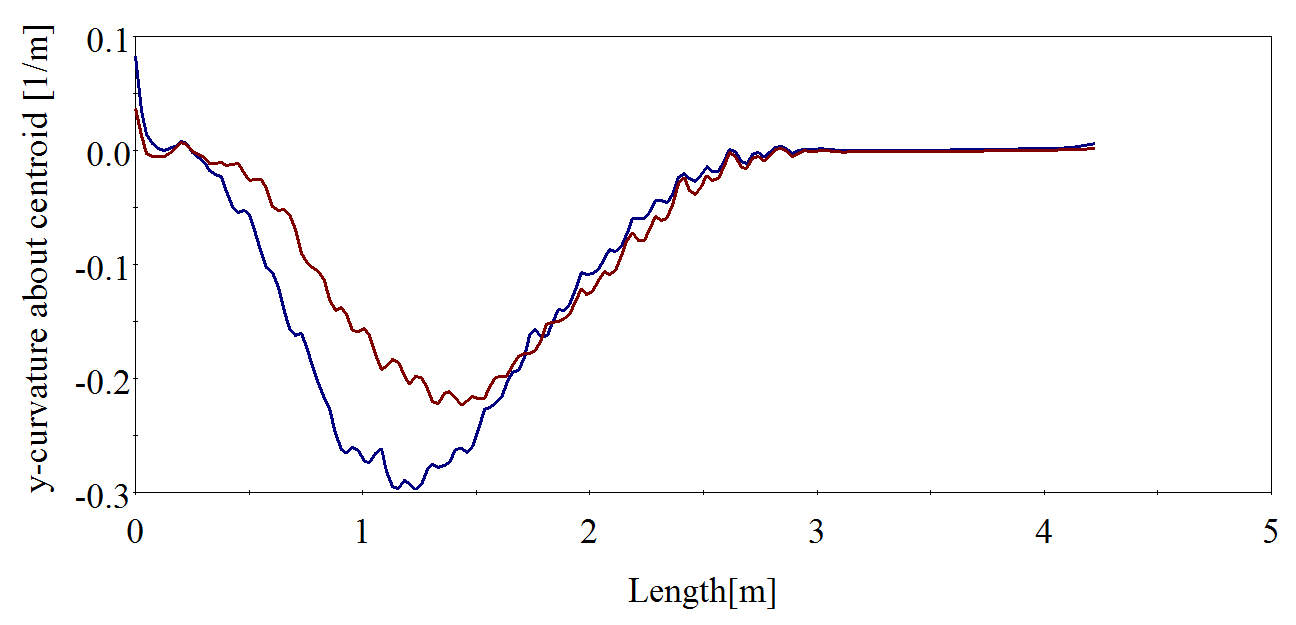
\includegraphics[width=.45\linewidth]{figures/c1}}\hfill
\caption[$\; \:$Results from load Case 1]{Results from load Case 1. The blue plot is at the maximum angle and the red plot is at the minimum angle}
\label{fig:r1}
\end{figure}

\begin{figure}[H]
\subfloat[Tension in conductor \label{fig:f2}]
  {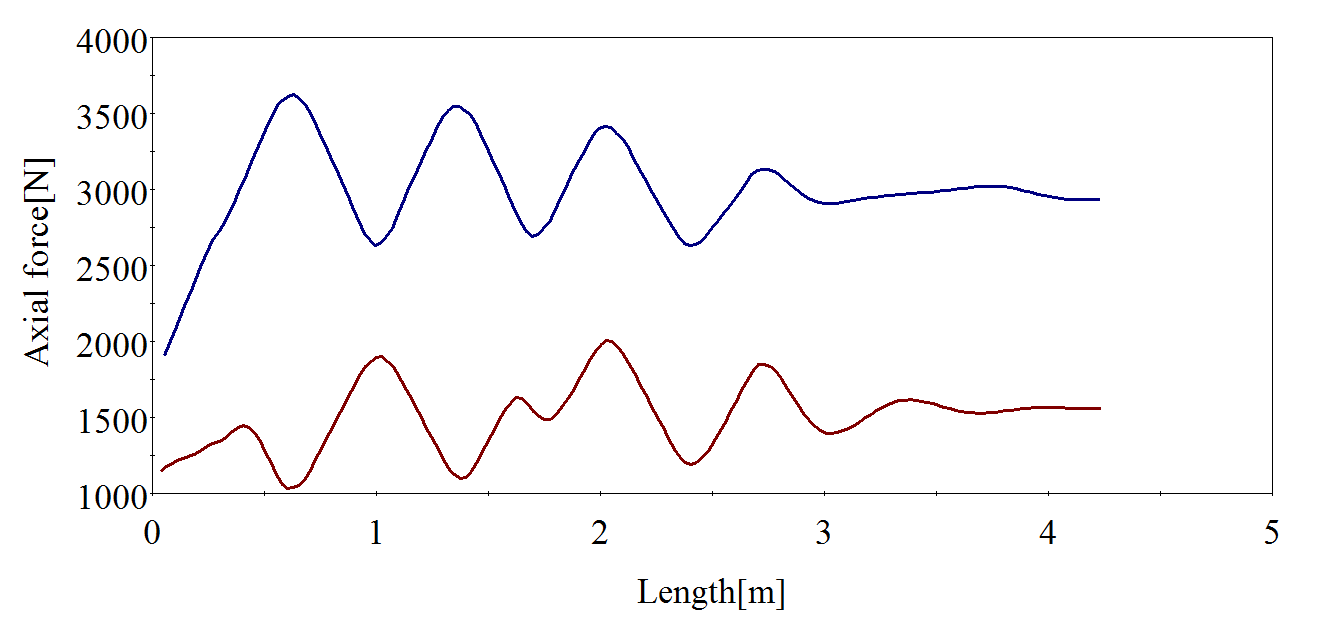
\includegraphics[width=.45\linewidth]{figures/f2}}\hfill
\subfloat[Curvature in conductor \label{fig:c2}]
  {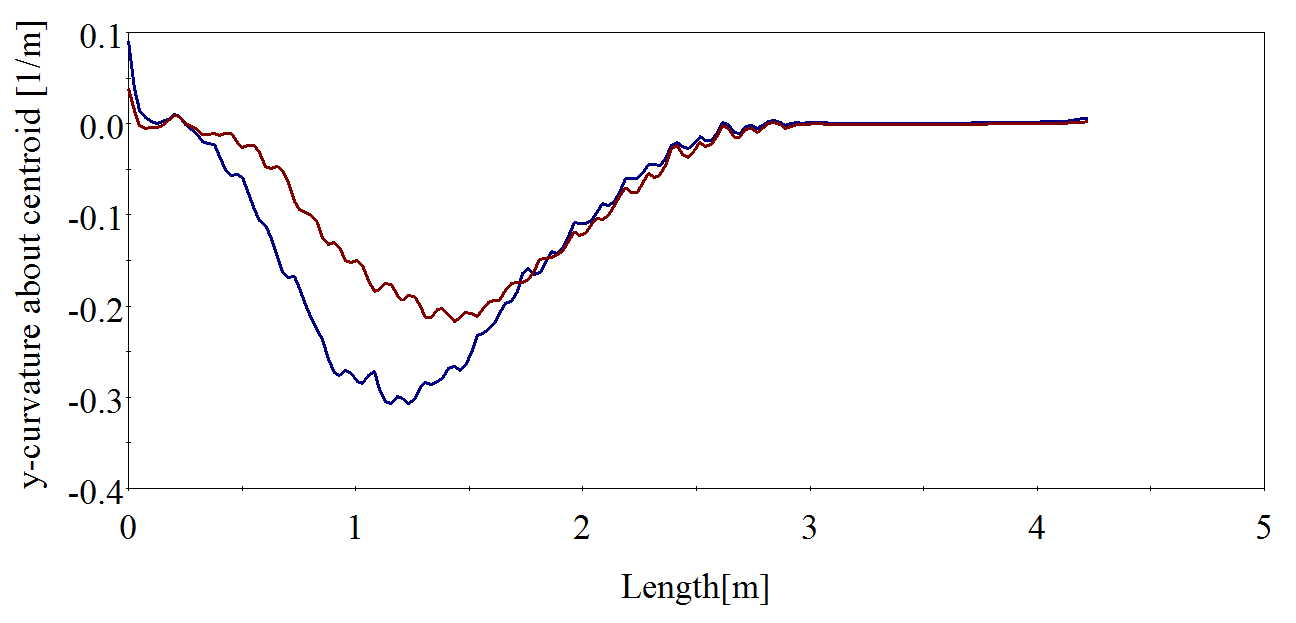
\includegraphics[width=.45\linewidth]{figures/c2}}\hfill
\caption[$\; \:$Results from load Case 2]{Results from load Case 2. The blue plot is at the maximum angle and the red plot is at the the minimum angle}
\label{fig:r2}
\end{figure}

\begin{figure}[H]
\subfloat[Tension in conductor \label{fig:f3}]
  {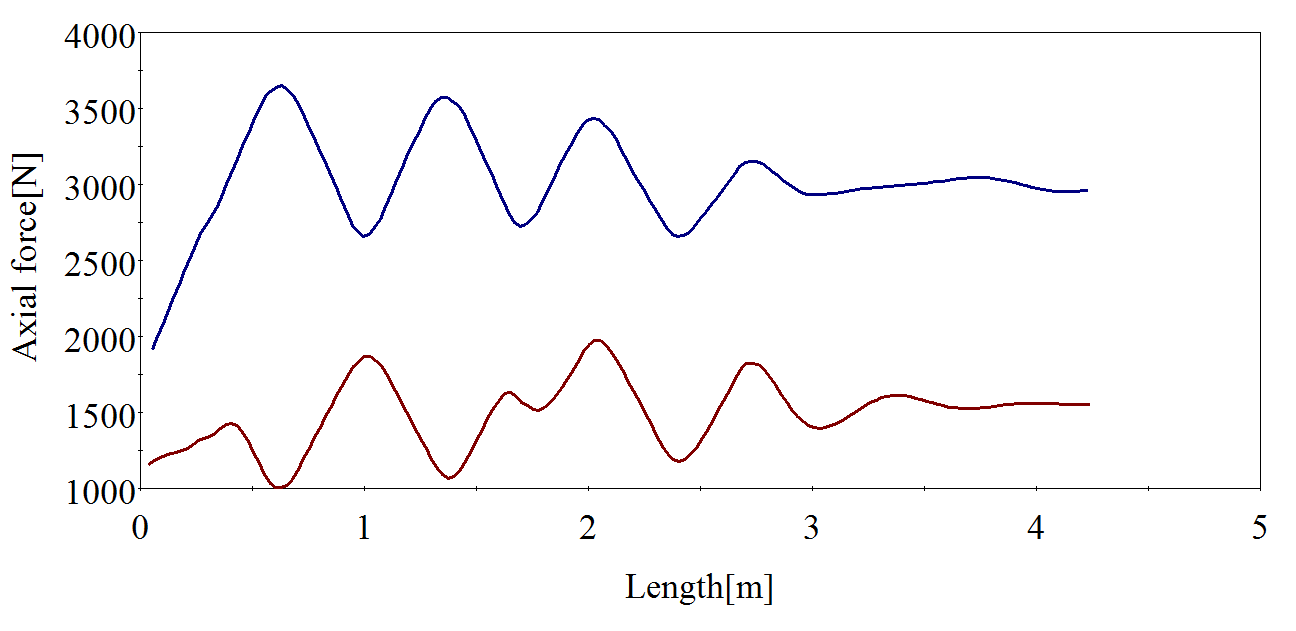
\includegraphics[width=.45\linewidth]{figures/f3}}\hfill
\subfloat[Curvature in conductor \label{fig:c3}]
  {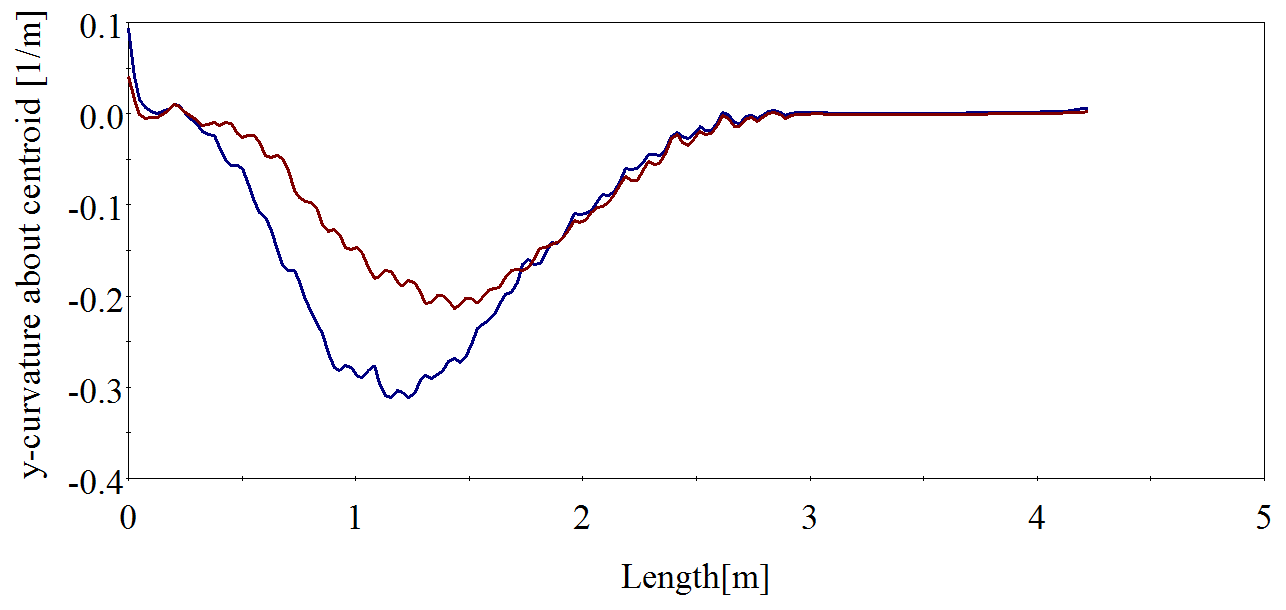
\includegraphics[width=.45\linewidth]{figures/c3}}\hfill
\caption[$\; \:$Results from load Case 3]{Results from load Case 3. The blue plot is at the maximum angle and the red plot is at the the minimum angle}
\label{fig:r3}
\end{figure}

\begin{figure}[H]
\subfloat[Tension in conductor \label{fig:f4}]
  {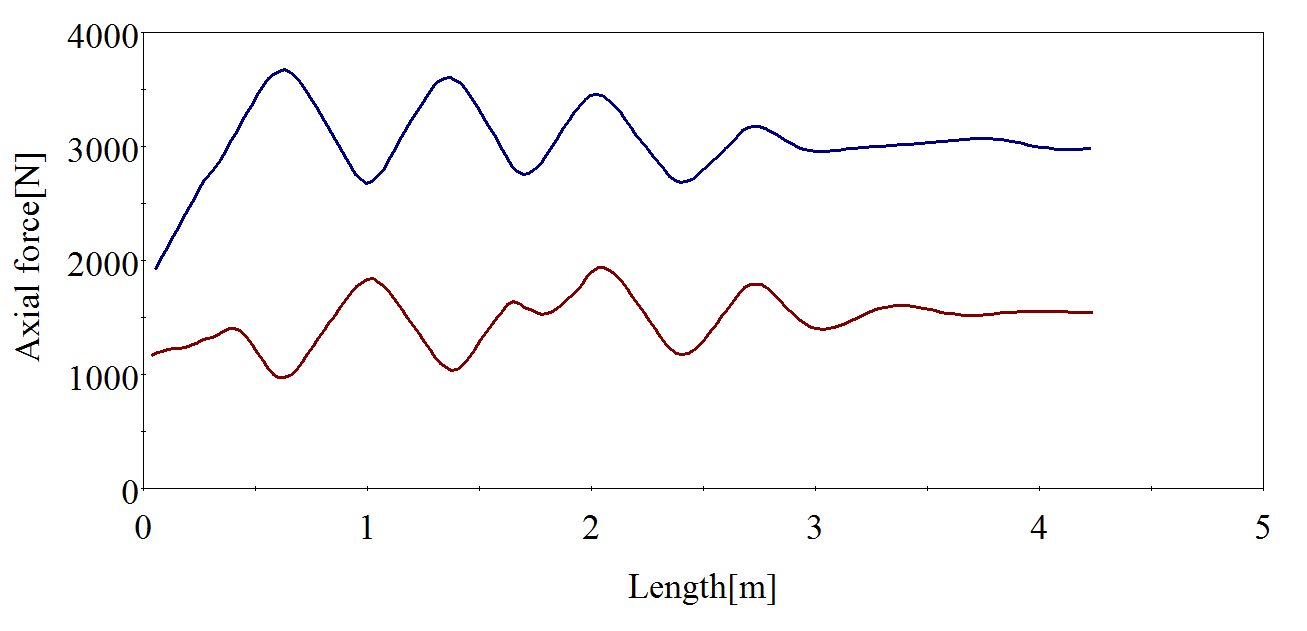
\includegraphics[width=.45\linewidth]{figures/f4}}\hfill
\subfloat[Curvature in conductor \label{fig:c4}]
  {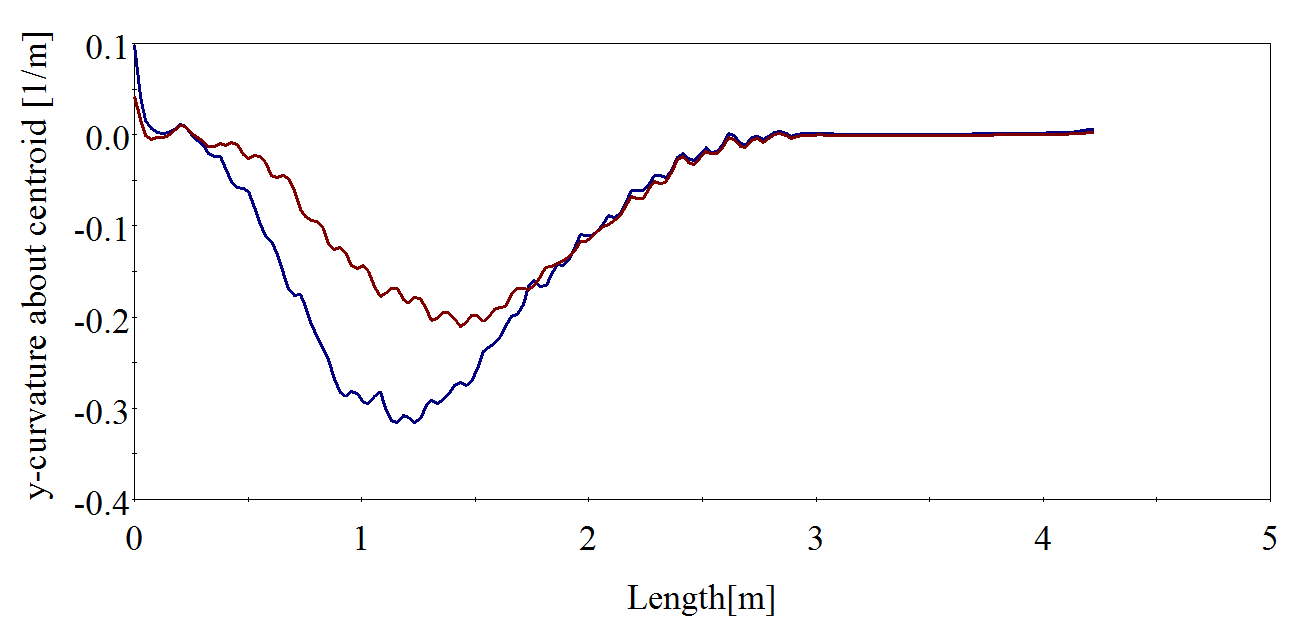
\includegraphics[width=.45\linewidth]{figures/c4}}\hfill
\caption[$\; \:$Results from load Case 4]{Results from load Case 4. The blue plot is at the maximum angle and the red plot is at the the minimum angle}
\label{fig:r4}
\end{figure}

\begin{figure}[H]
\subfloat[Tension in conductor \label{fig:f5}]
  {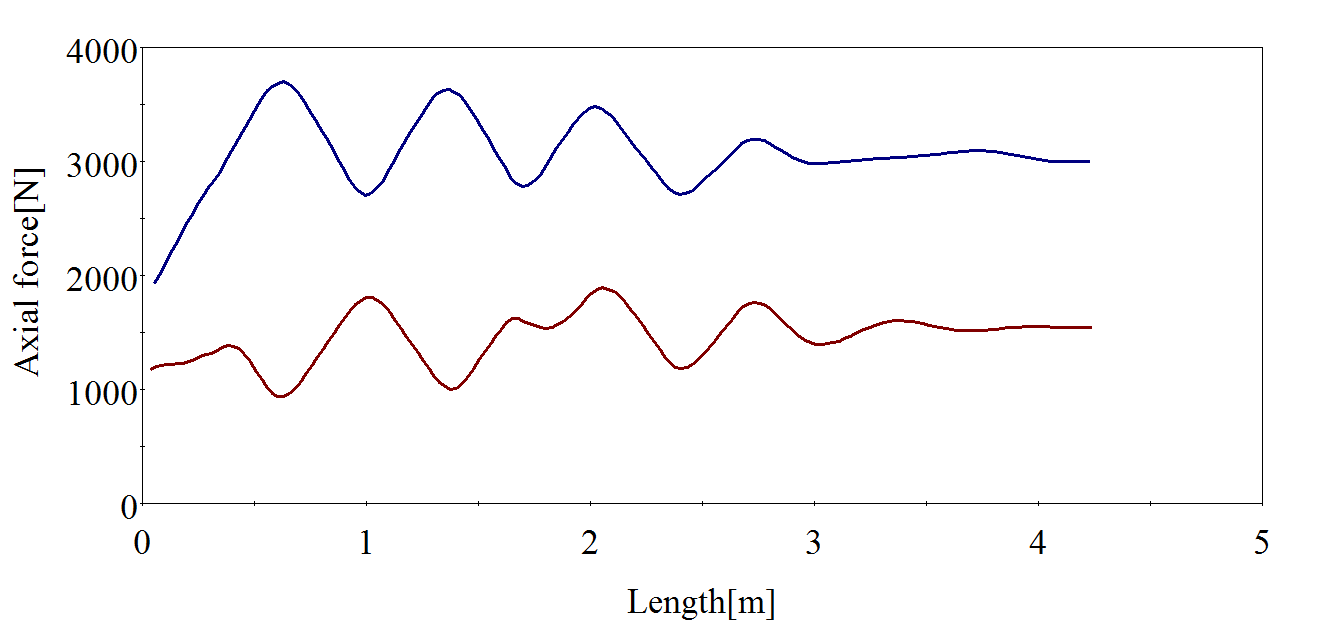
\includegraphics[width=.45\linewidth]{figures/f5}}\hfill
\subfloat[Curvature in conductor \label{fig:c5}]
  {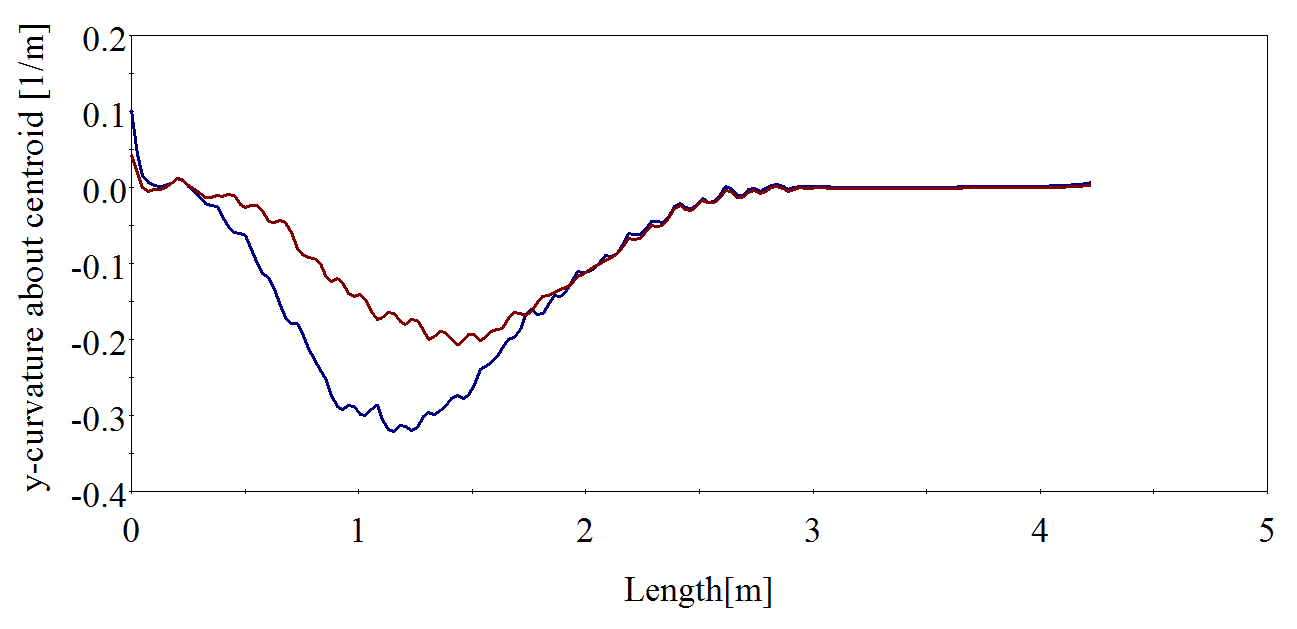
\includegraphics[width=.45\linewidth]{figures/c5}}\hfill
\caption[$\; \:$Results from load Case 5]{Results from load Case 5. The blue plot is at the maximum angle and the red plot is at the the minimum angle}
\label{fig:r5}
\end{figure}

\begin{figure}[H]
\subfloat[Tension in conductor \label{fig:f6}]
  {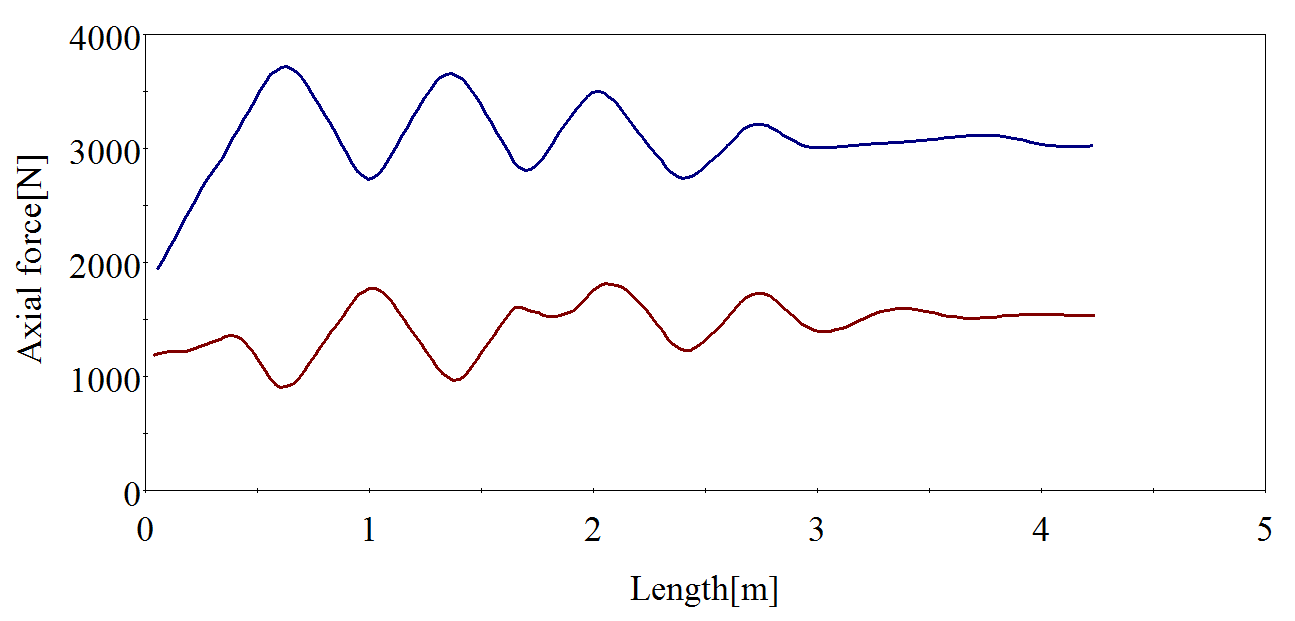
\includegraphics[width=.45\linewidth]{figures/f6}}\hfill
\subfloat[Curvature in conductor \label{fig:c6}]
  {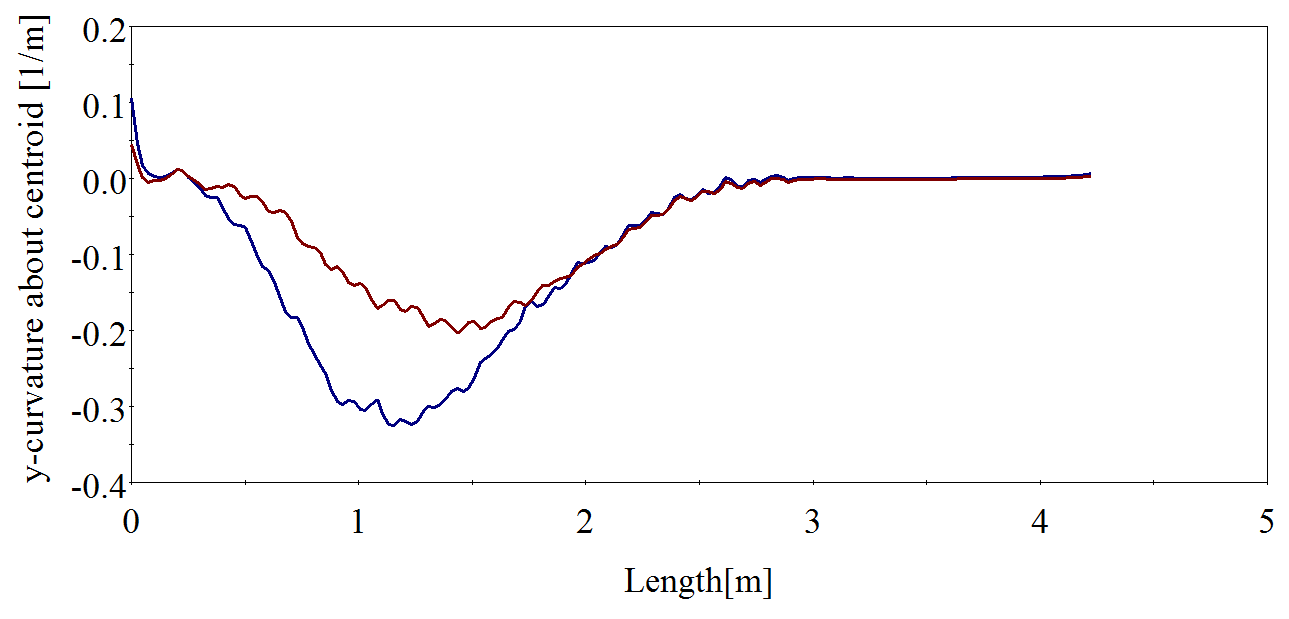
\includegraphics[width=.45\linewidth]{figures/c6}}\hfill
\caption[$\; \:$Results from load Case 6]{Results from load Case 6. The blue plot is at the maximum angle and the red plot is at the the minimum angle}
\label{fig:r6}
\end{figure}

\begin{figure}[H]
\subfloat[Tension in conductor \label{fig:f7}]
  {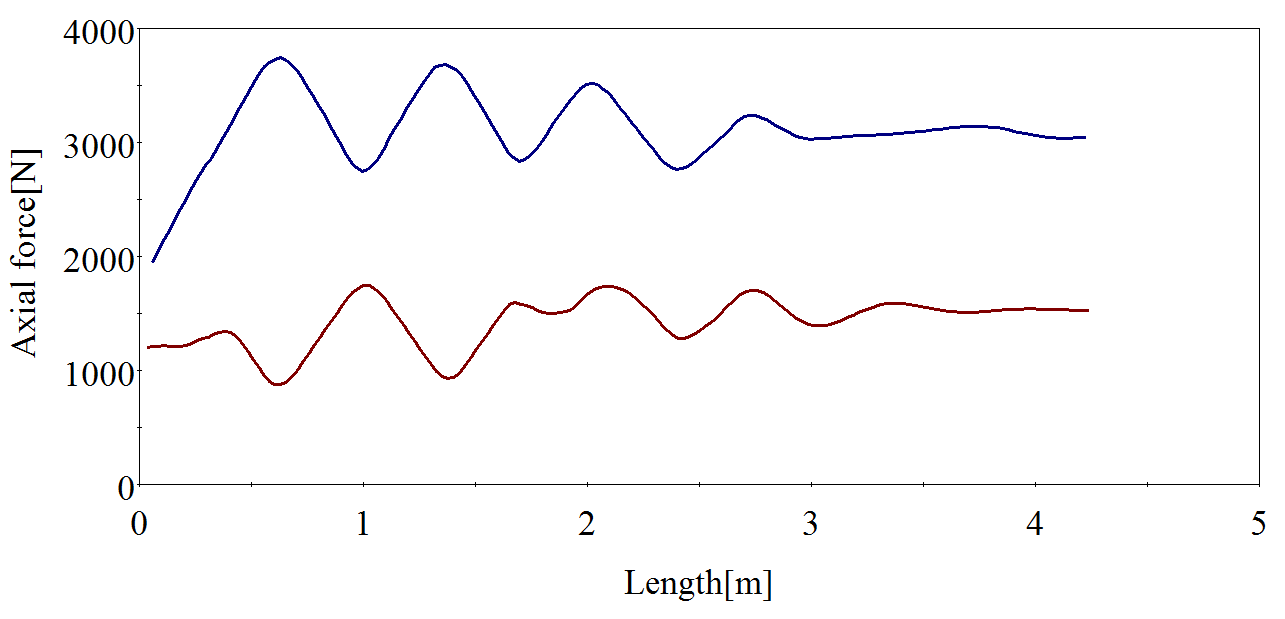
\includegraphics[width=.45\linewidth]{figures/f7}}\hfill
\subfloat[Curvature in conductor \label{fig:c7}]
  {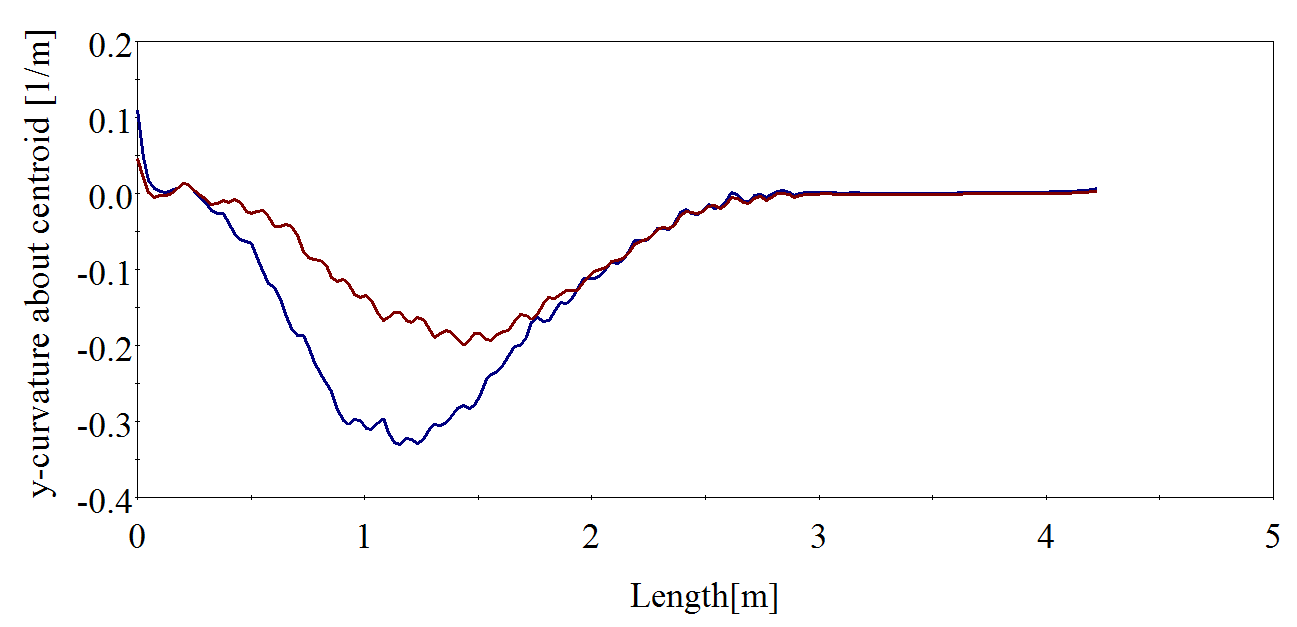
\includegraphics[width=.45\linewidth]{figures/c7}}\hfill
\caption[$\; \:$Results from load Case 7]{Results from load Case 7. The blue plot is at the maximum angle and the red plot is at the the minimum angle}
\label{fig:r7}
\end{figure}

\begin{figure}[H]
\subfloat[Tension in conductor \label{fig:f8}]
  {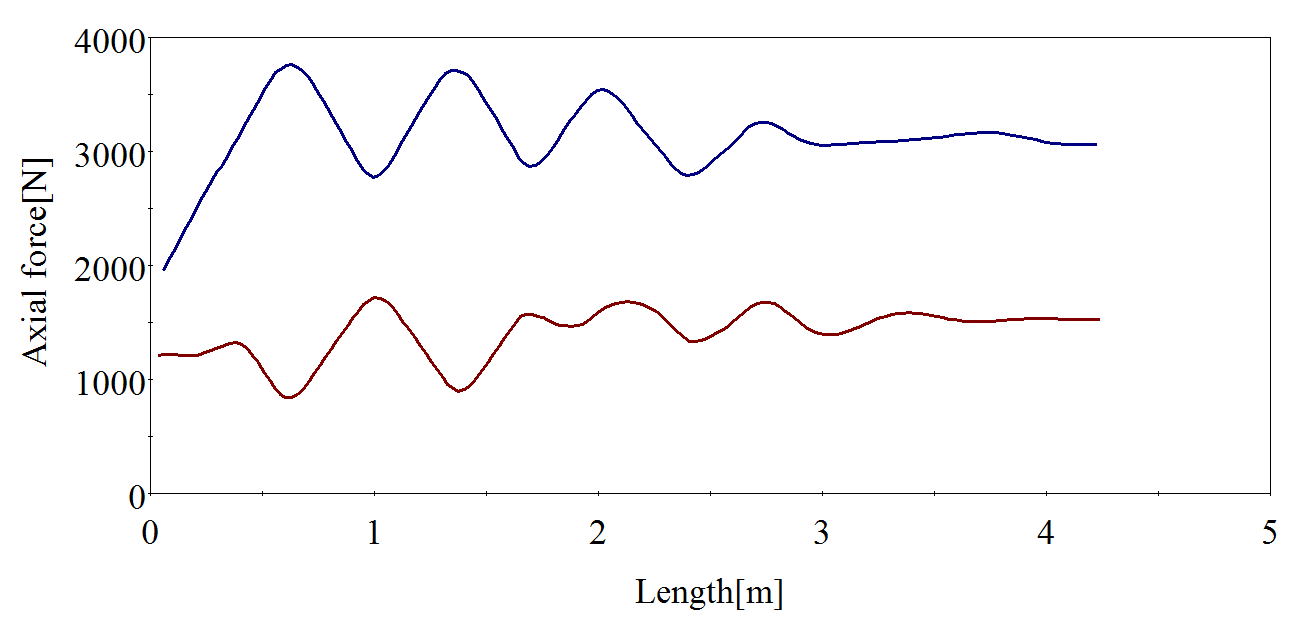
\includegraphics[width=.45\linewidth]{figures/f8}}\hfill
\subfloat[Curvature in conductor \label{fig:c8}]
  {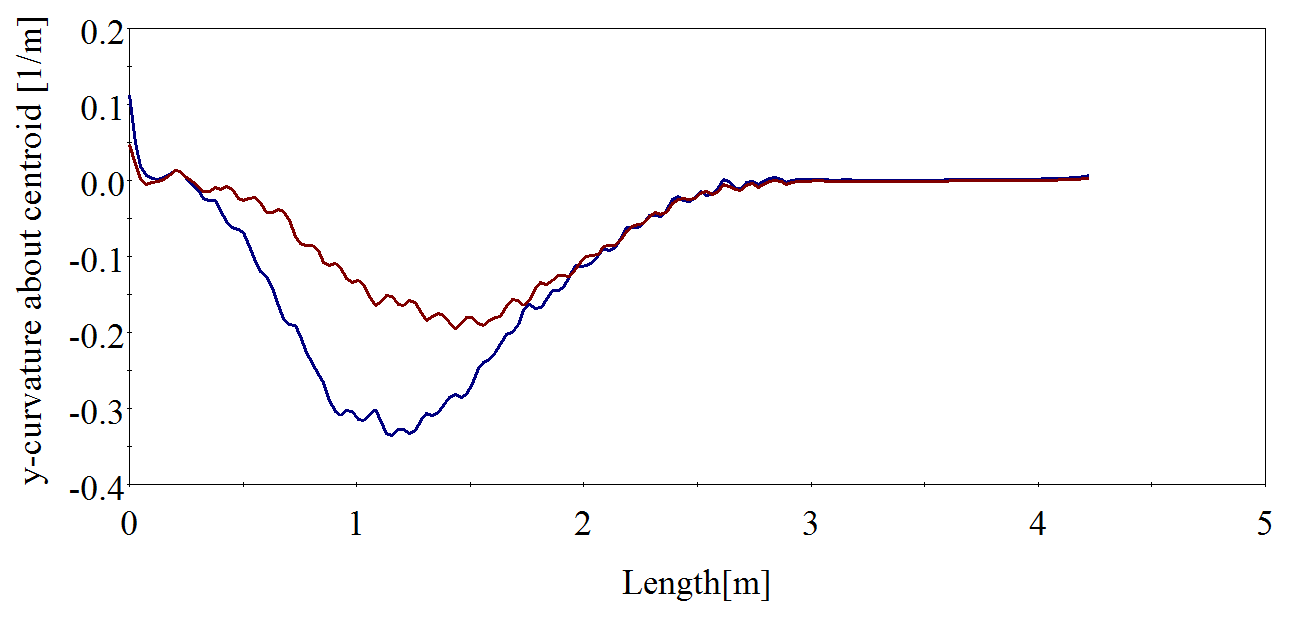
\includegraphics[width=.45\linewidth]{figures/c8}}\hfill
\caption[$\; \:$Results from load Case 8]{Results from load Case 8. The blue plot is at the maximum angle and the red plot is at the the minimum angle}
\label{fig:r8}
\end{figure}

\begin{figure}[H]
\subfloat[Tension in conductor \label{fig:f9}]
  {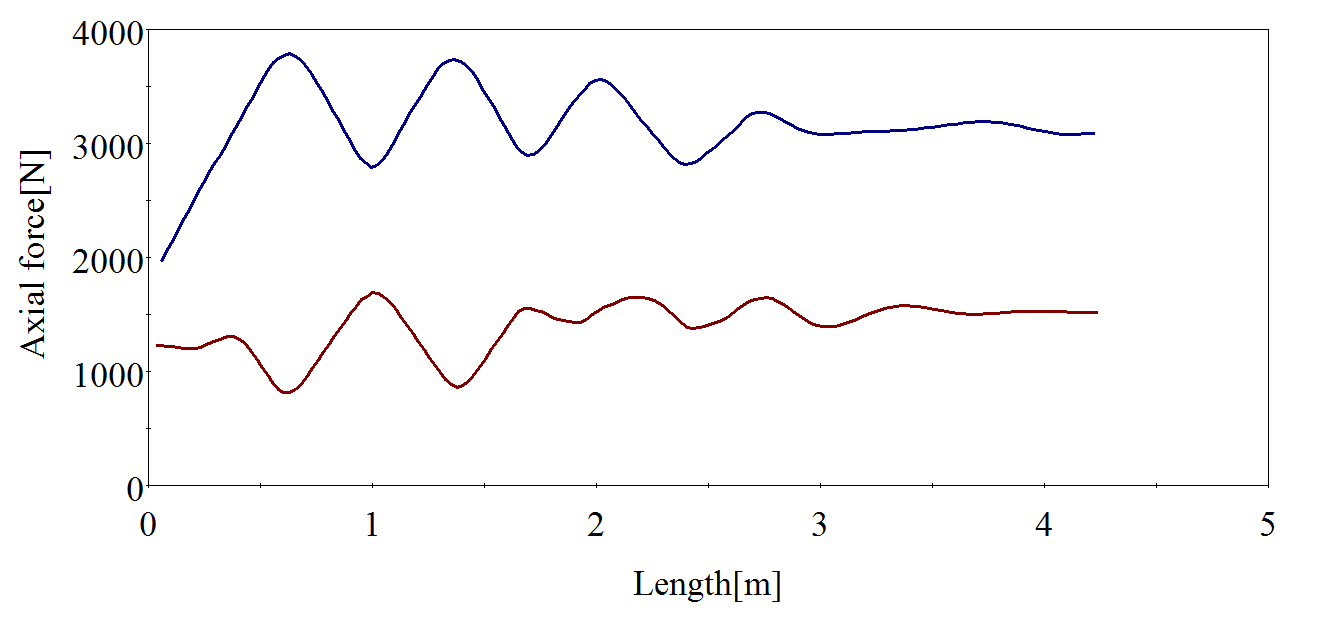
\includegraphics[width=.45\linewidth]{figures/f9}}\hfill
\subfloat[Curvature in conductor \label{fig:c9}]
  {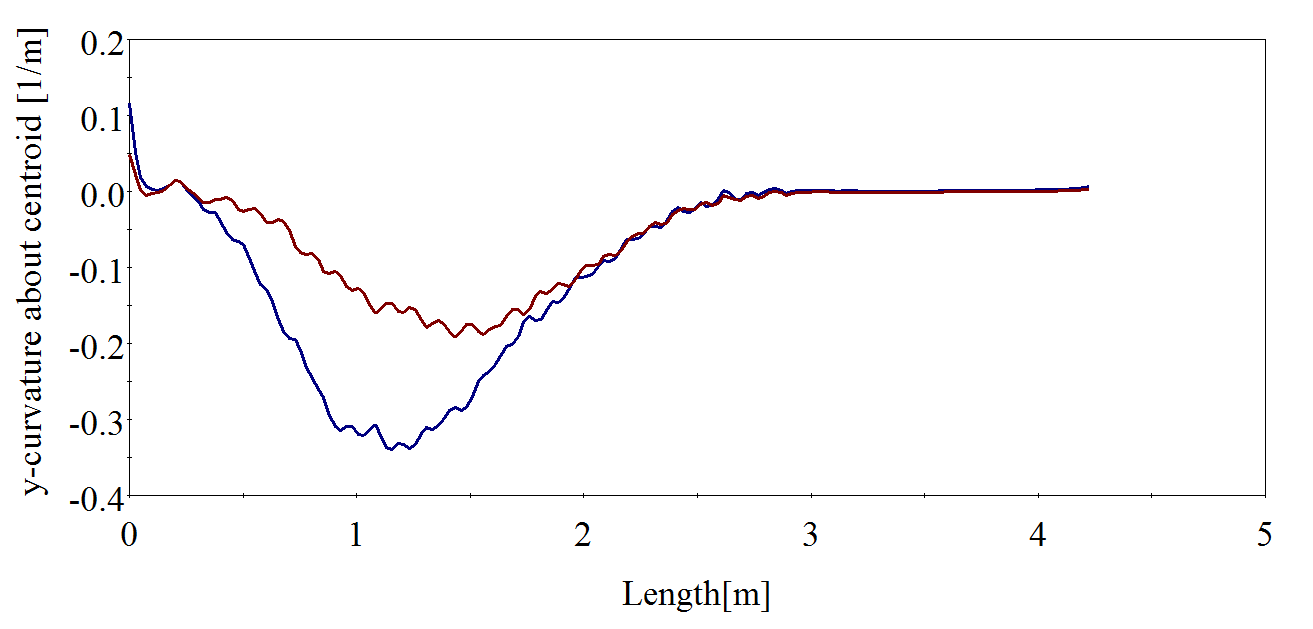
\includegraphics[width=.45\linewidth]{figures/c9}}\hfill
\caption[$\; \:$Results from load Case 9]{Results from load Case 9. The blue plot is at the maximum angle and the red plot is at the the minimum angle}
\label{fig:r9}
\end{figure}

\begin{figure}[H]
\subfloat[Tension in conductor \label{fig:f10}]
  {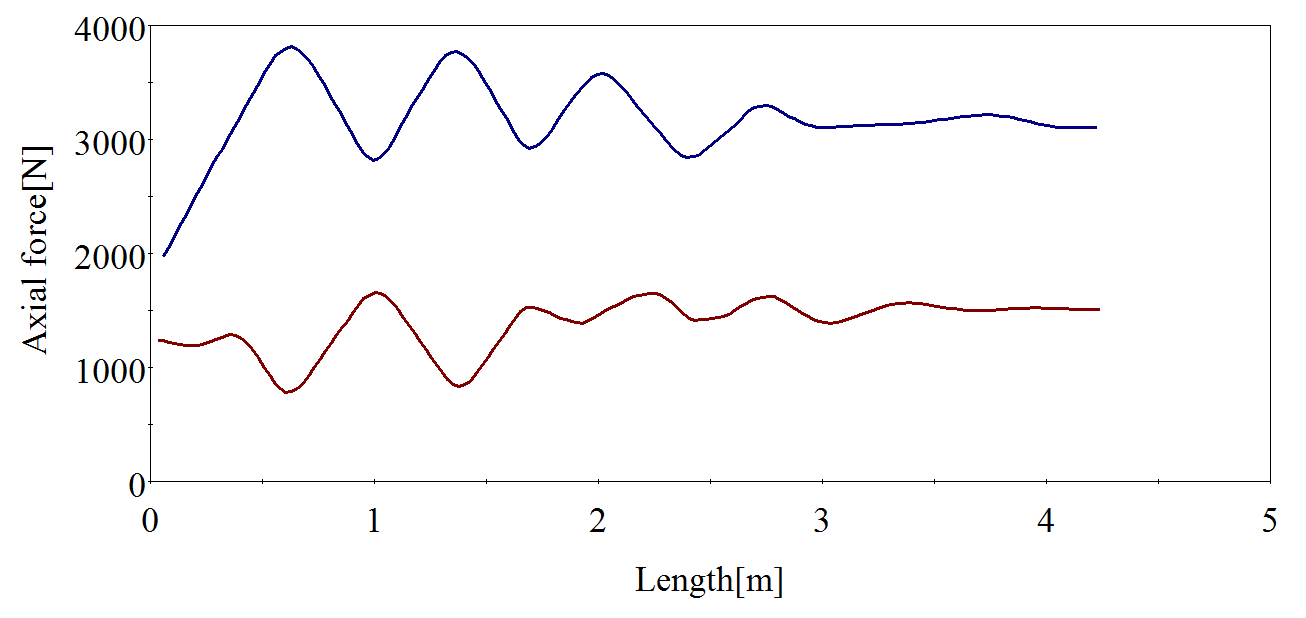
\includegraphics[width=.45\linewidth]{figures/f10}}\hfill
\subfloat[Curvature in conductor \label{fig:c10}]
  {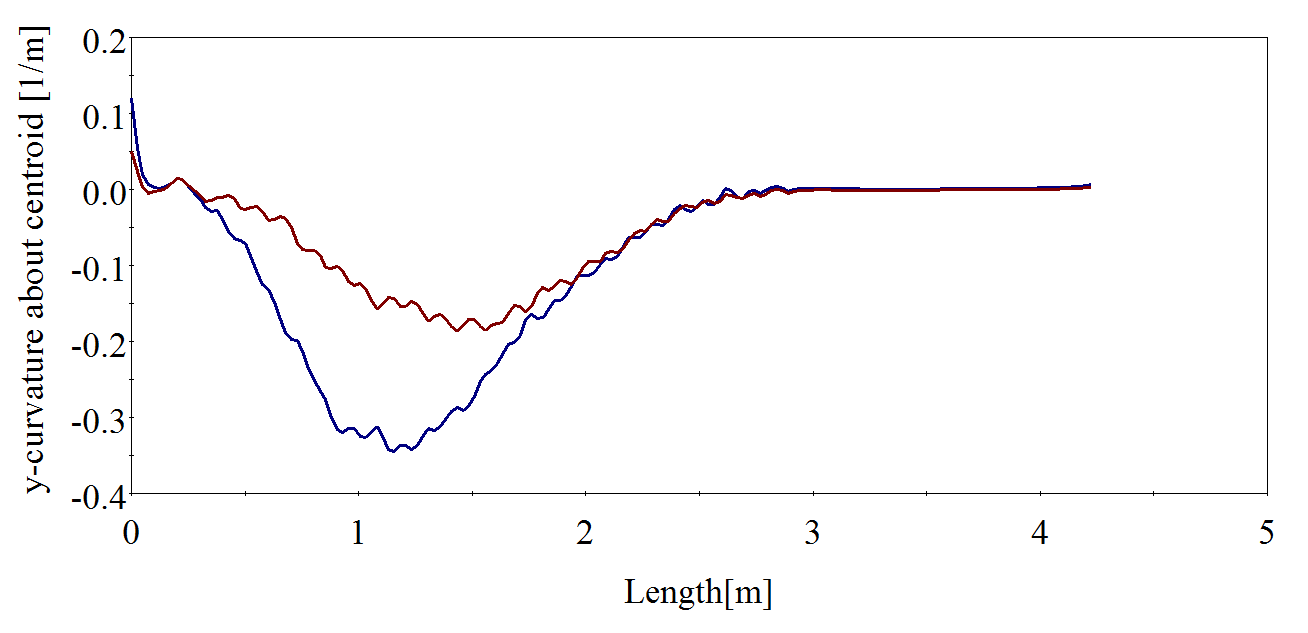
\includegraphics[width=.45\linewidth]{figures/c10}}\hfill
\caption[$\; \:$Results from load Case 10]{Results from load Case 10. The blue plot is at the maximum angle and the red plot is at the the minimum angle}
\label{fig:r10}
\end{figure}

\begin{figure}[H]
\subfloat[Tension in conductor \label{fig:f11}]
  {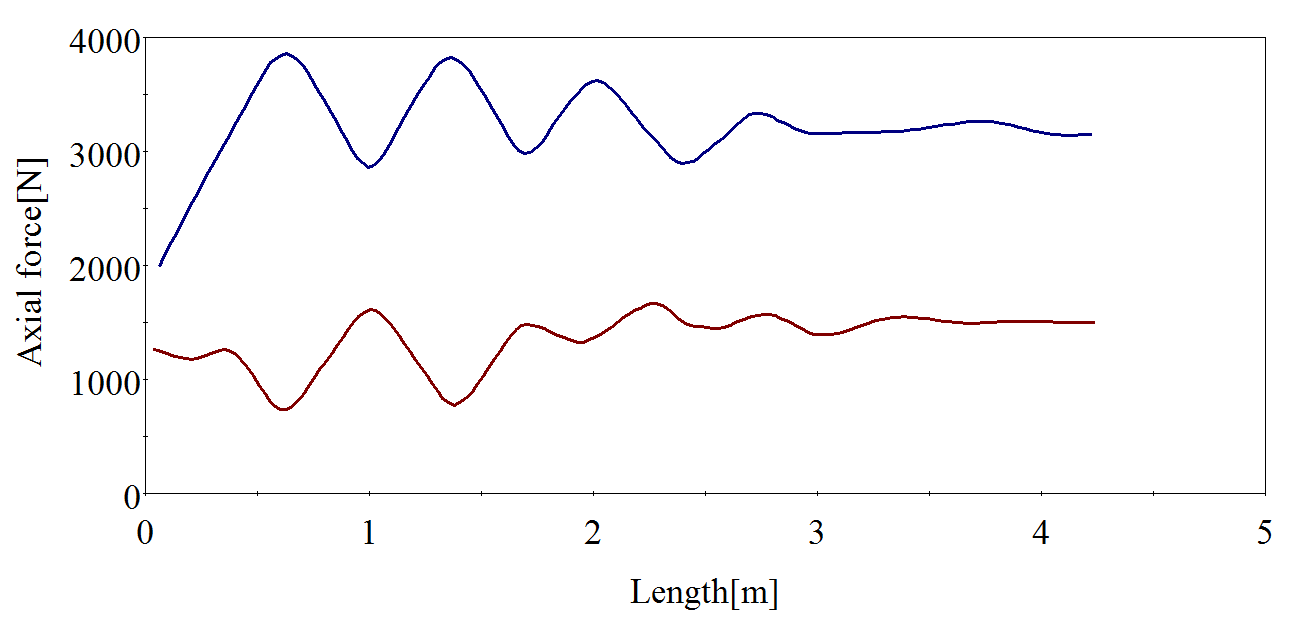
\includegraphics[width=.45\linewidth]{figures/f11}}\hfill
\subfloat[Curvature in conductor \label{fig:c11}]
  {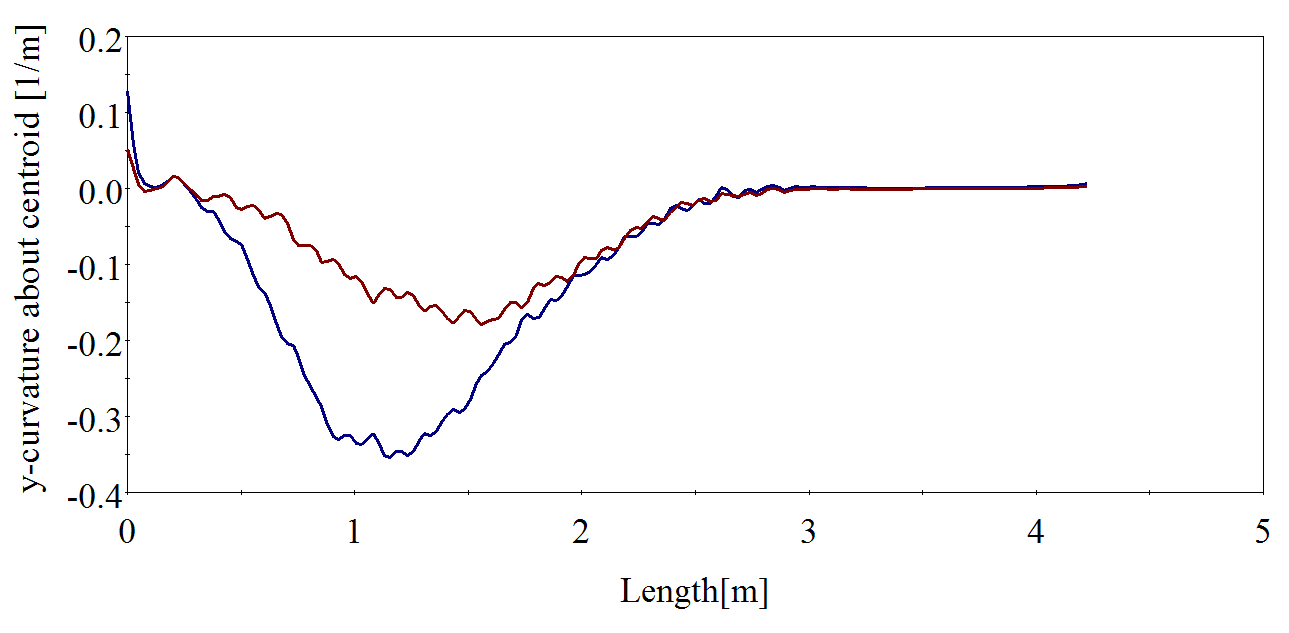
\includegraphics[width=.45\linewidth]{figures/c11}}\hfill
\caption[$\; \:$Results from load Case 11]{Results from load Case 11. The blue plot is at the maximum angle and the red plot is at the the minimum angle}
\label{fig:r11}
\end{figure}

\begin{figure}[H]
\subfloat[Tension in conductor \label{fig:f12}]
  {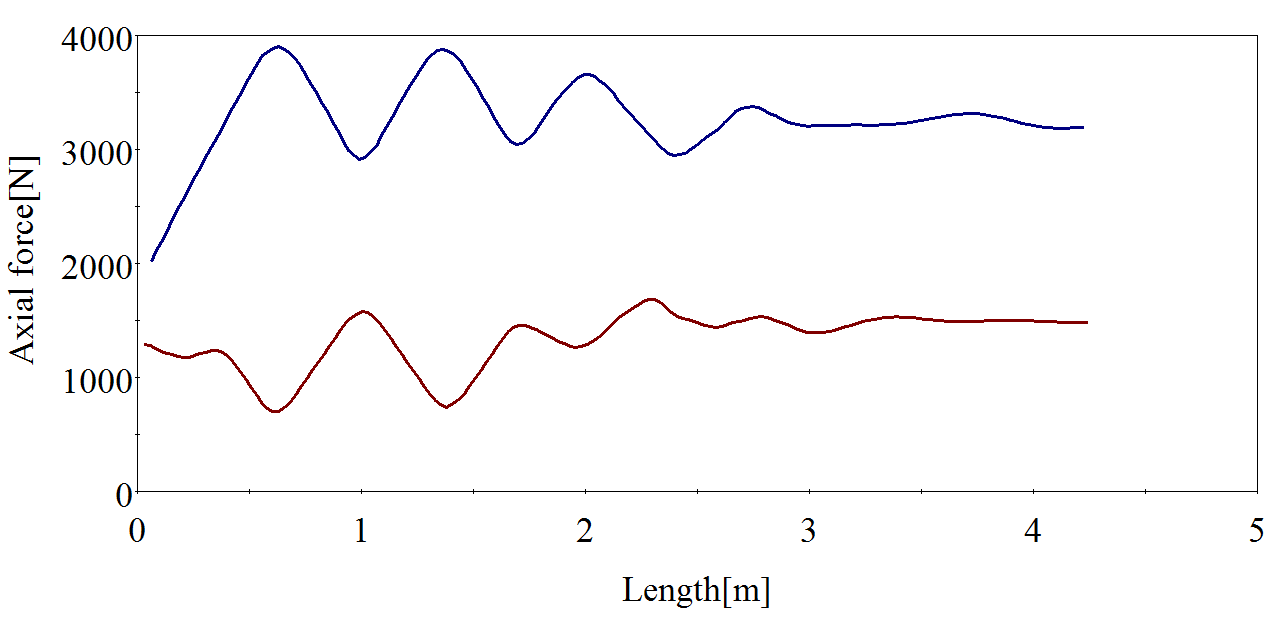
\includegraphics[width=.45\linewidth]{figures/f12}}\hfill
\subfloat[Curvature in conductor \label{fig:c12}]
  {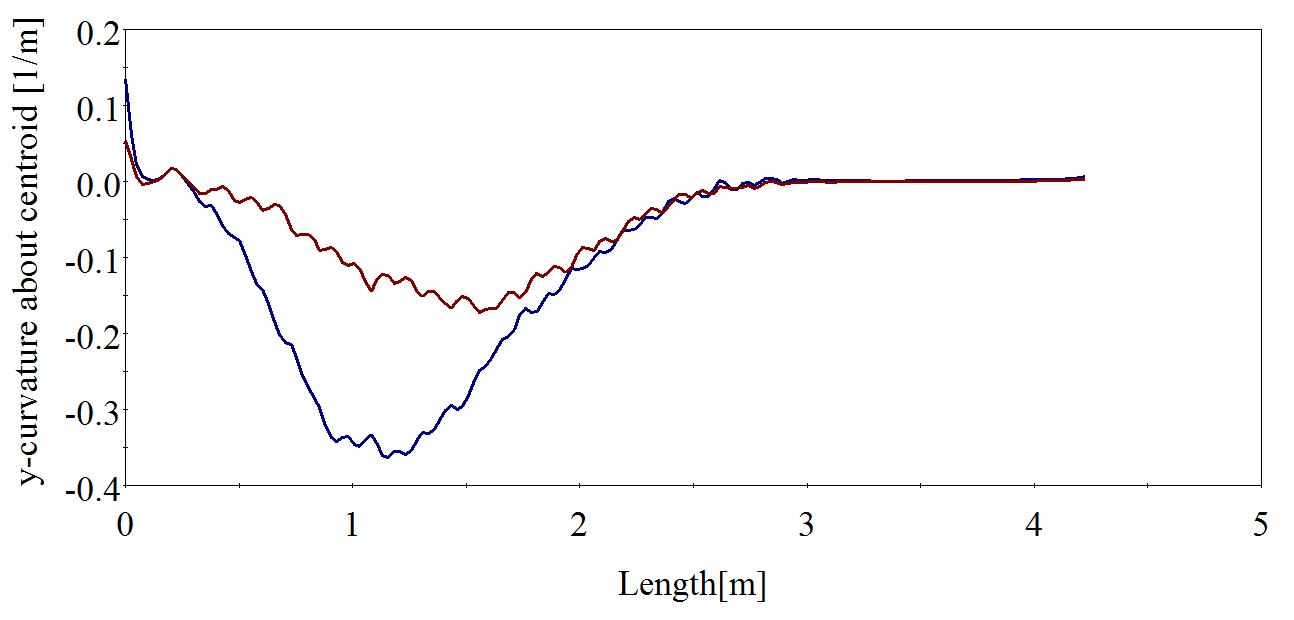
\includegraphics[width=.45\linewidth]{figures/c12}}\hfill
\caption[$\; \:$Results from load Case 12]{Results from load Case 12. The blue plot is at the maximum angle and the red plot is at the the minimum angle}
\label{fig:r12}
\end{figure}

\begin{figure}[H]
\subfloat[Tension in conductor \label{fig:f13}]
  {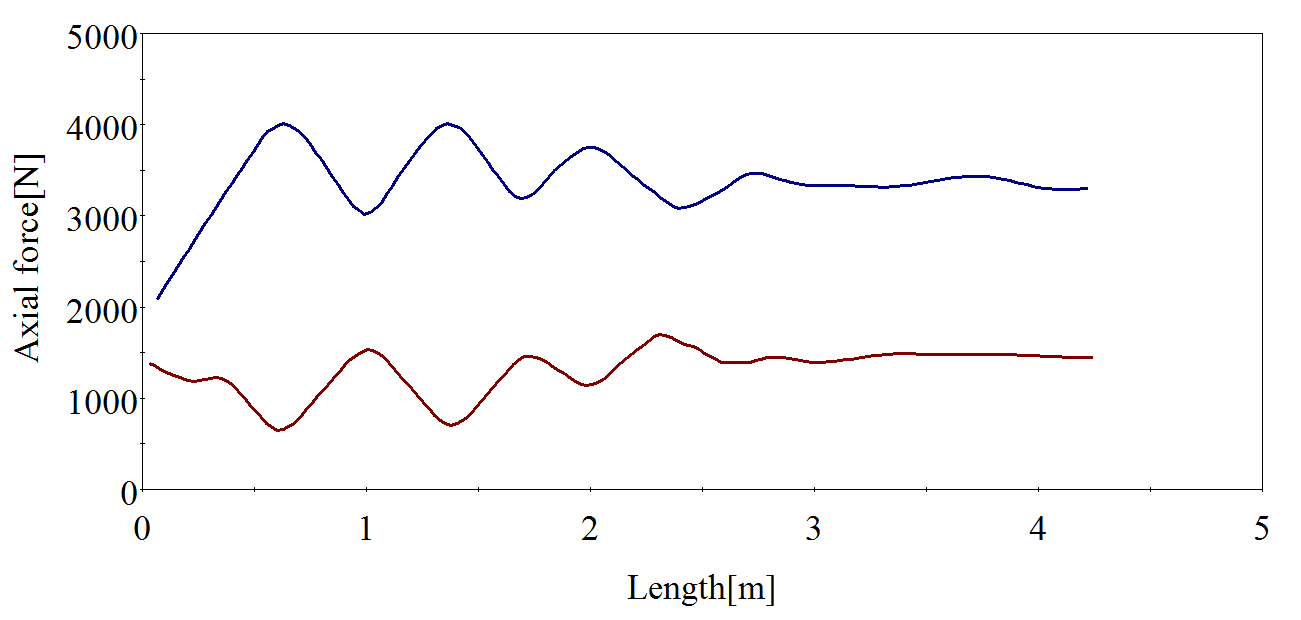
\includegraphics[width=.45\linewidth]{figures/f13}}\hfill
\subfloat[Curvature in conductor \label{fig:c13}]
  {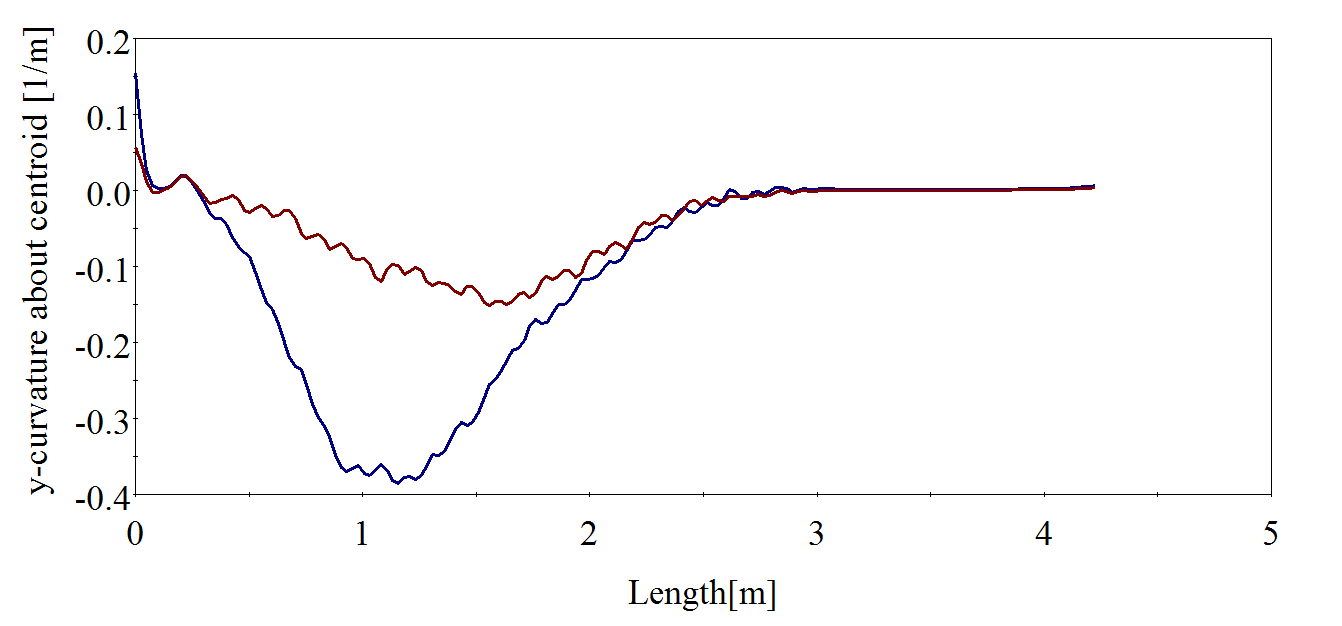
\includegraphics[width=.45\linewidth]{figures/c13}}\hfill
\caption[$\; \:$Results from load Case 13]{Results from load Case 13. The blue plot is at the maximum angle and the red plot is at the the minimum angle}
\label{fig:r13}
\end{figure}

\begin{figure}[H]
\subfloat[Tension in conductor \label{fig:f14}]
  {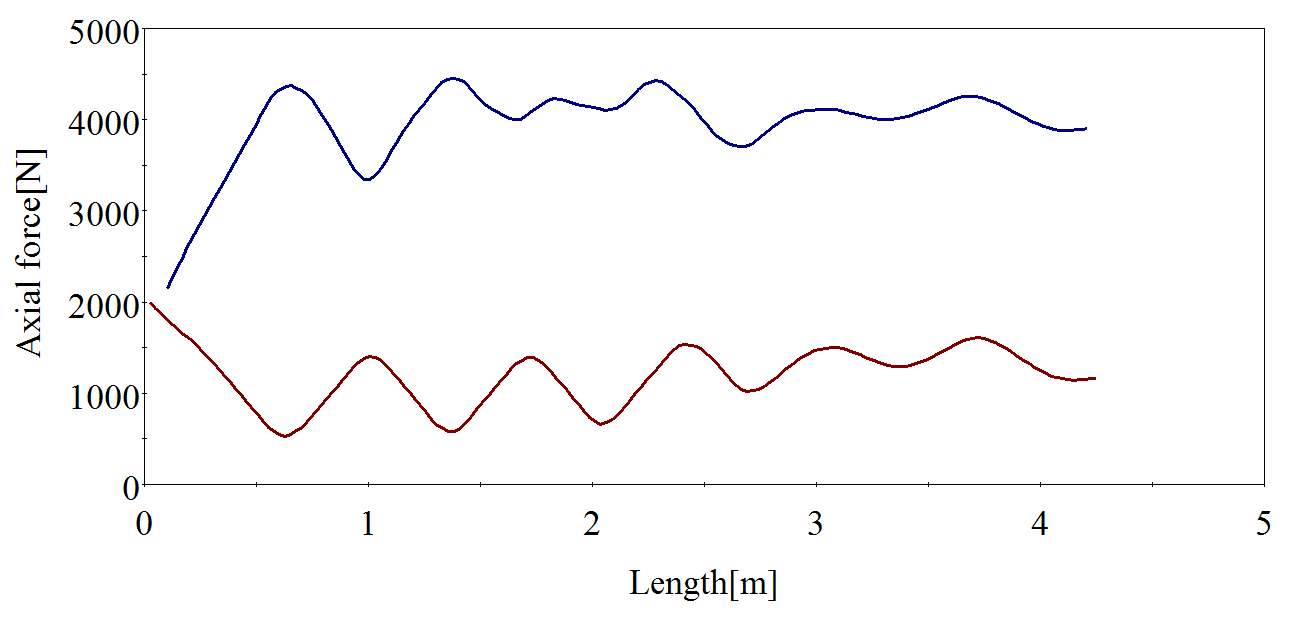
\includegraphics[width=.45\linewidth]{figures/f14}}\hfill
\subfloat[Curvature in conductor \label{fig:c14}]
  {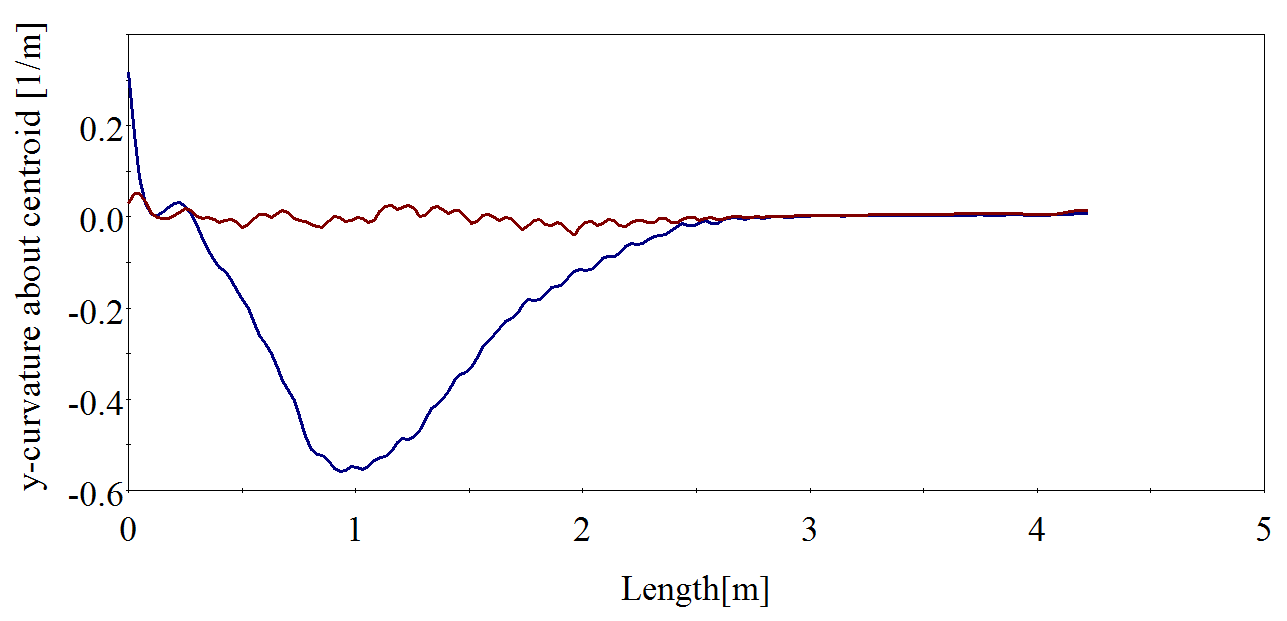
\includegraphics[width=.45\linewidth]{figures/c14}}\hfill
\caption[$\; \:$Results from load Case 14]{Results from load Case 14. The blue plot is at the maximum angle and the red plot is at the the minimum angle}
\label{fig:r14}
\end{figure}

\begin{figure}[H]
\subfloat[Tension in conductor \label{fig:f15}]
  {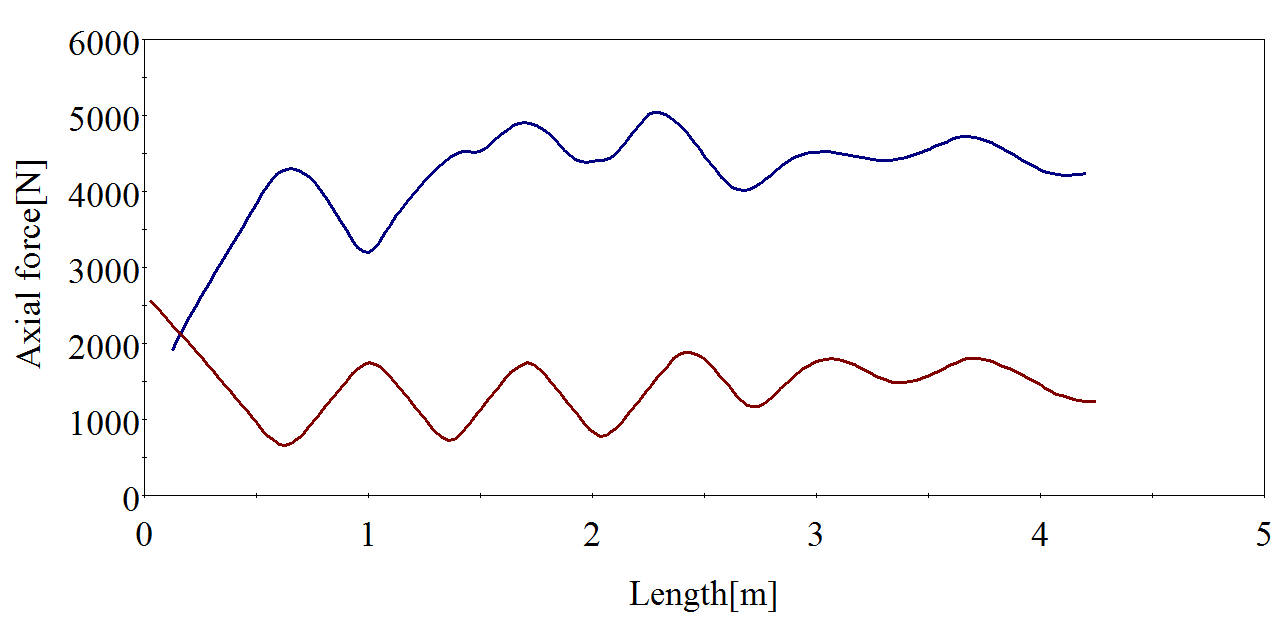
\includegraphics[width=.45\linewidth]{figures/f15}}\hfill
\subfloat[Curvature in conductor \label{fig:c15}]
  {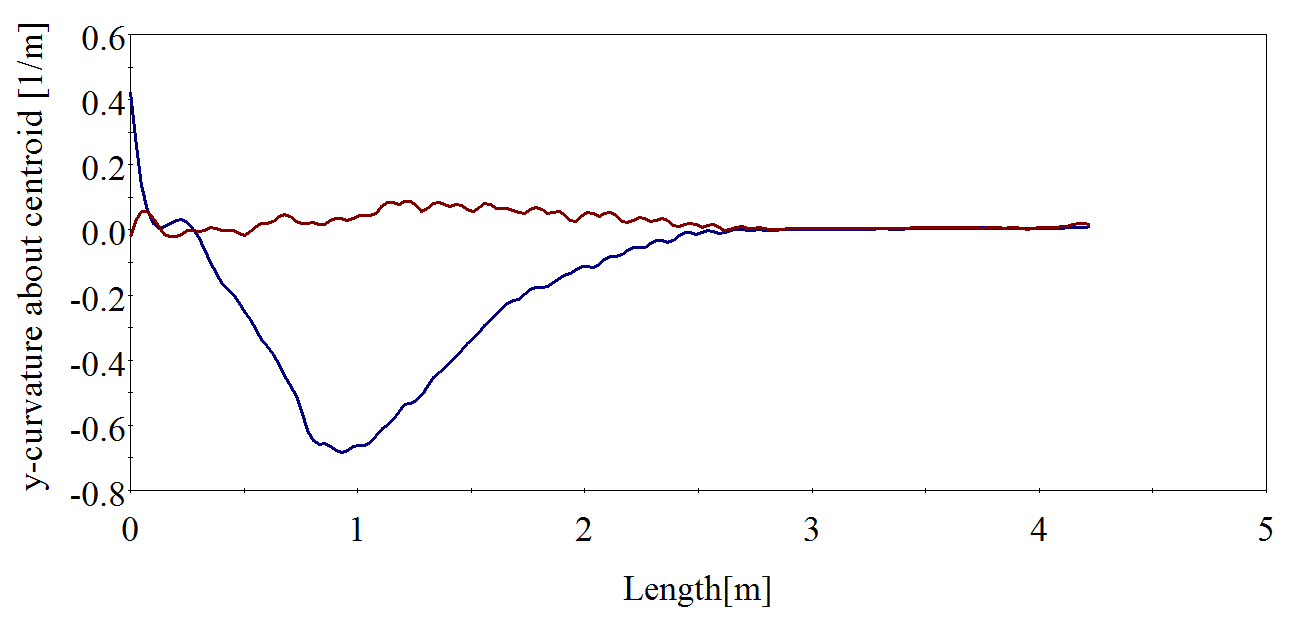
\includegraphics[width=.45\linewidth]{figures/c15}}\hfill
\caption[$\; \:$Results from load Case 15]{Results from load Case 15. The blue plot is at the maximum angle and the red plot is at the the minimum angle}
\label{fig:r15}
\end{figure}